\chapter{Homology}
A summary of Hatcher's homology section from his \emph{Algebraic Topology}
book.
\section{Simplicial and Signular Homology}
Skip all this nonsense. I need to catch up.
\section{Computations and Applications}
\subsection{Degree}
For a map $f\colon S^n\to S^n$ with $n>0$, the induced map $f_*\colon
H_n(S^n)\to H_n(S^n)$ is a homomorphism from an infinite cyclic group to
itself and so must be of the form $f_*(\alpha)=df(\alpha)$ for some integer
$d$ depending only on $f$. This integer is called the \emph{degree} of $f$
and is denoted by $\deg f$. Here are some basic properties of the degree
\begin{enumerate}[label=(\arabic*)]
\item $\deg\id_{S^n}=1$ since $(\id_{S^n})_*=\id_{H_n(S^n)}$.
\item $\deg f=0$ if $f$ is not injective. For if we choose a point $x_0\in
  S^n\minus f(S^n)$ then $f$ can be factored as a composition $S^n\to
  S^n\minus\{x_0\}\hookrightarrow S^n$ and $H_n(S^n\minus\{x_0\})=0$ since
  $S^n\minus\{x_0\}$ is contractible.
\item If $f\simeq g$ then $\deg f=\deg g$ since $f_*=g_*$. The converse
  statement, that if $\deg f=\deg g$, is a fundamental theorem of Hopf from
  around 1925 which we prove in Corollary 4.25.
\item $\deg fg=\deg f\deg g$, since $(f\circ g)_*=f_*\circ g_*$. As a
  consequence, $\deg f=\pm 1$ if $f$ is a homotopy equivalence since
  $f\circ g\simeq \id_{S^n}$ implies that $\deg f\deg g=\deg\id_{S^n}=1$.
\item $\deg f=-1$ if $f$ is a reflection of $S^n$, fixing the points in
  some subsphere $S^{n-1}\subset S^n$ and interchanging the two
  complementary hemispheres. For we can give $S^n$ a $\Delta$-complex
  structure with these two hemispheres as its two $n$-simplices
  $\Delta_1^n$ and $\Delta_2^n$, and the $n$-chain $\Delta_1^n-\Delta_2^n$
  represents a generator of $H_n(S^n)$ as we saw in Example 2.23, so the
  reflection interchanging $\Delta_1^n$ and $\Delta_2^n$ sends this
  generator to its negative.
\item The antipodal map $a\colon S^n\to S^n$, $x\mapsto -x$, has degree
  $(-1)^{n+1}$ since it is the composition of $n+1$ reflections, each
  changing the sign of one coordinate in $\bfR^{n+1}$.
\item If $f\colon S^n\to S^n$ has no fixed points then $\deg
  f=(-1)^{n+1}$. For if $f(x)\neq x$ for any $x\in S^n$, then the line
  segment from $f(x)$ to $-x$, defined by $t\mapsto(1-t)f(x)-tx$ for $0\leq
  t\leq 1$, does not pass through the origin. Hence if $f$ has no fixed
  points, the formula $f_t(x)\coloneqq[(1-t)f(x)-tx]/\|(1-t)f(x)-tx\|$
  defines a homotopy from $f$ to the antipodal map. Note that the antipodal
  map has no fixed points, so the fact that maps without fixed points are
  homotopic to the antipodal point is sort of a converse statement.
\end{enumerate}
\begin{theorem}[2.8]
$S^n$ has a continuous field of nonzero tangent vectors if and only if $n$
is odd.
\end{theorem}
\begin{proposition*}[2.29]
$\bfZ/2\bfZ$ is the only nontrivial group that can act freely on $S^n$ if
$n$ is even.
\end{proposition*}

Recall that the action of a group $G$ on a space $X$ is a homomorphism from
$G$ to the group $\Homeo(X)$ of homeomorphisms $X\to X$, and the action is
free if the homeomorphism corresponding to each nontrivial element of $G$
has no fixed points. In the case of $S^n$, the antipodal map $x\mapsto -x$
generates a free action of $\bfZ/2\bfZ$.

Next we describe a technique for computing degrees which can be applied to
most maps that arise in practice. Suppose $f\colon S^n\to S^n$, $n>0$, has
the property that for some point $y\in S^n$, the preimage $f^{-1}(y)$
consists of only finitely many points, say $x_1,\dotsc,x_m$. Let
$U_1,\dotsc,U_m$ be disjoint neighborhoods of these points, mapped by $f$
into a neighborhood $V$ of $y$. Then $f(U_i\minus\{x_i\})\subset
V\minus\{y_i\}$ for each $i$, and we have a commutative diagram
\[
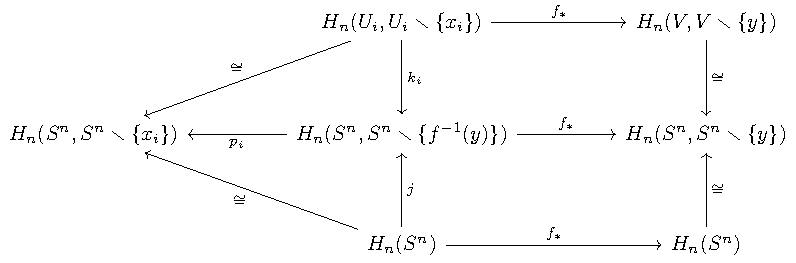
\includegraphics{figures/notes-degree-disjoint-neighborhoods}
\]
where all the maps are the obvious ones, and in particular $k_i$ and $p_i$
are induced by inclusions, so the triangles and squares commute. The two
isomorphisms in the upper half of the diagram come from excision, while the
lower two isomorphisms come from exact sequences of pairs. Via these four
isomorphisms, the top two groups in the diagram can be identified with
$H_n(S^n)\cong\bfZ$, and the top homomorphism $f_*$ becomes multiplication
by an integer called the \emph{local degree} of $f$ at $x_i$, written $\deg
f|_{x_i}$.

For example, if $f$ is a homeomorphism, then $y$ can be any point and there
is only one corresponding to $x_i$, so all the maps in the diagram are
isomorphisms and $\deg f|_{x_i}=\deg f=\pm 1$. The situation occurs quite
often in applications, and it is usually not hard to determine the correct
signs.

Here is the formula that reduces degree calculations to computing local
degrees:
\begin{proposition}[2.30]
$\deg f=\sum_i\deg f|_{x_i}$.
\end{proposition}
\begin{proof}
By excision the central term $H_n(S^n,S^n\minus\{f^{-1}(y)\})$ in the
preceding lemma is the direct sum of the groups
$H_n(U_i,U_i\minus\{x_i\})\cong\bfZ$, with $k_i$ the inclusion of the
$i$-th  summand and $p_i$ the projection onto the $i$th
summand. Identifying the outer groups in the diagram with $\bfZ$ as before,
commutativity of the lower triangle says that that $p_i\circ j(1)=1$, hence
$j(1)=(1,\dotsc,1)=\sum_ik_i(1)$. Commutativity of the upper square says
that the middle $f_*$ takes $k_i(1)$ to $\deg f|_{x_i}$, hence the sum
$\sum_ik_i(1)$ is taken to $\sum_i\deg f|_{x_i}$. Commutativity of the
lower square then gives the formula $\deg f=\sum_i\deg f|_{x_i}$.
\end{proof}
\begin{example}[2.31]
We can use this result to construct a map $S^n\to S^n$ of any given degree,
for each $n\geq 1$. Let $q\colon S^n\to \bigvee_k S^n$ be the quotient map
obtained by collapsing the complement of $k$ disjoint open balls $B_i$ in
$S^n$ to a point, and let $p\colon\bigvee_k S^n\to S^n$ identifying all the
summands to a single
\end{example}

%%% Local Variables:
%%% mode: latex
%%% TeX-master: "../MA572-Notes"
%%% End:
